\chapter{Preliminary Graph Theory}\label{ch:prelim}

First, let's define some basic concepts of graph theory, starting with the graph itself.

\section{Graphs}

A graph is an algebraic structure most commonly used to describe relationships between objects. There are many definitions of a graph, the most abstract being simply a set $V$ and a relation $R$ on $V$ denoting which elements of $V$ are connected. Graphs in general are \textit{directed}; if $R$ is symmetric, the graph is \textit{undirected}. For the purposes of this work we will be using a geometric definition and generally undirected graphs.
An undirected graph is an ordered pair $G = (V, E)$, where $V$ is a set of \textit{vertices} and $E$ is a set of \textit{edges}, i. e. a set of unordered pairs of vertices $\forall e \in E: ~ e = (u,v); u,v \in V$.
A \textit{path} in a graph $G$ from $v$ to $w$; $v,w \in V$ is a sequence of vertices $(u_1, u_2, \dots, u_n); ~ \{u_i ~|~ 1 \leq i \leq n\} \subseteq V$ such that $u_1 = v$, $u_n = w$ and $\{(u_i, u_{i+1}) ~|~ 1 \leq i \leq n-1\} \subseteq E$. A graph is \textit{connected} if there exists a path between every pair of vertices $v,w \in V; ~ v \neq w$.
A \textit{degree} $\Delta (v)$ of a vertex $v$ denotes how many edges are incident to this vertex. $\Delta(G)$ is the highest degree of any vertex in $G$.
A graph is \textit{k-regular} if the degree of each vertex is exactly $k$. A \textit{cubic graph} is a 3-regular graph.

As an example, a complete graph with 4 vertices $K_4$ is cubic.

\begin{figure}[h]
    \centering
        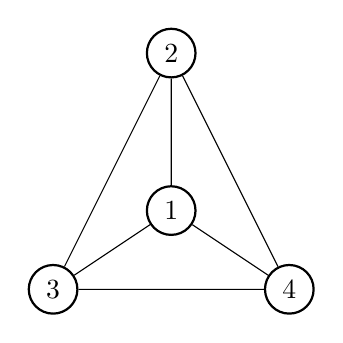
\begin{tikzpicture}
            \begin{scope}[every node/.style={circle,thick,draw}]
                \node (1) at (0,0) {1};
                \node (2) at (0,2) {2};
                \node (3) at (-1.5,-1) {3};
                \node (4) at (1.5,-1) {4};
            \end{scope}
            \draw (1) -- (2) -- (3) -- (4) -- (1) (2) -- (4) (1) -- (3);
        \end{tikzpicture}
\end{figure}

In general statements about graphs in later chapters we are referring to unordered cubic graphs.

\subsection{Colouring}

When simple binary relationships between objects are not enough, weighted graphs and colouring offer a wider range of applications. Assigning colours to vertices or edges of graphs makes classifications of these objects possible.
A vertex colouring of a graph $G$ is a mapping from the vertex set of $G$ to a set of colours $C$. An edge colouring of a graph $G$ is a mapping from the edge set of $G$ to a set of colours $C$.
A \textit{proper vertex colouring} of $G$ is a vertex colouring such that no two neighboring vertices share a colour. A \textit{proper edge colouring} is an edge colouring such that no two edges that share an endpoint have the same colour. A proper colouring using $k$ colours is called a \textit{$k$-colouring}.

As colouring in general is not very interesting, we will be considering only proper colourings henceforth. It is also important to define the set of "colours", especially when colouring signed graphs. It is most practical to use a subset of integers $C \subseteq \mathbb{Z}$ because it makes definitions and proofs clear. Additionally, it is important that a $k$-colouring uses a set of $k$ colours.

The canonical colouring problem is to find the minimum number of colours required for a proper colouring. This number is called the \textit{chromatic number} for vertex colourings and \textit{chromatic index} for edge colourings. Determining the chromatic number and index is useful in other areas of graph theory as well.

\begin{theorem}\label{th:bipartite}
    A graph is bipartite if and only if it has a proper vertex 2-colouring.
\end{theorem}

For regular unsigned graphs these numbers are known.

\begin{theorem}[Brooks\cite{brooks}]
    The chromatic number of a graph $G$ is $\Delta(G)$ for all graphs except complete graphs and cycles of odd length, where the chromatic number is $\Delta(G) + 1$.
\end{theorem}

\begin{theorem}[Vizing]
    The chromatic index of a simple graph $G$ is $\Delta(G)$ or $\Delta(G) + 1$.
\end{theorem}

In other words, we can always colour the edges of a graph using at most $\Delta(G) + 1$ colours where $\Delta(G)$ is the highest degree of any vertex in $G$. The lower bound $\Delta(G)$ is trivial; we need exactly $\Delta(G)$ colours at the highest degree vertex in $G$ to construct a proper colouring. The Vizing theorem proves the upper bound using Kempe chains.

\section{Signed graphs}

A signed graph is a graph in which each edge has either a positive or a negative sign. There are multiple definitions of a signed graph, we will be mostly using a pair of an unsigned graph and a sign function:
A \textit{signed graph} $\Gamma = (G, \sigma)$ consists of a \textit{underlying graph} $G$ and a \textit{sign function} $\sigma : E(G) \rightarrow \{+,-\}$ that assigns a sign to each edge of $G$.

\begin{figure}[h]
    \centering
        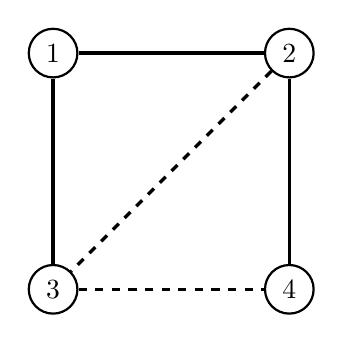
\begin{tikzpicture}
            \begin{scope}[every node/.style={circle,thick,draw}]
                \node (1) at (0,0) {1};
                \node (2) at (3,0) {2};
                \node (3) at (0,-3) {3};
                \node (4) at (3,-3) {4};
            \end{scope}
            \begin{scope}[every edge/.style={draw,very thick}]
                \path
                    (1) edge (2)
                    (2) edge [dashed] (3)
                    (3) edge (1)
                    (2) edge (4)
                    (3) edge [dashed] (4);
            \end{scope}
        \end{tikzpicture}
    \caption[Example of a signed graph]{Example of a signed graph. Dashed lines indicate negative edges, solid lines positive edges.}
\end{figure}

A fundamental concept in the theory of signed graphs is \textit{vertex switching}. Switching a vertex of a signed graph reverses the sign of each edge incident to it. More generally, switching a signed subgraph reverses the sign of each edge between a vertex subset and its complement.

We can prove by induction that a signed graph can be switched to an all-positive graph if and only if it is balanced. Both conditions in Harary's theorem apply to all all-positive graphs and graphs that can be switched from an all-positive graph. Consequently, all balanced graphs are equivalent to an all-positive graph, which is an alternative definition of a positive graph. Similarly, we call a graph \textit{antibalanced} if it is equivalent to an all-negative graph, (all cycles of even length in and antibalanced graph are positive and cycles of odd length are negative).

If a signed graph can be obtained from another signed graph by switching, they are considered \textit{equivalent}. For a single underlying graph, switching forms \textit{equivalence classes} of signed graphs. Within a single equivalence class all graphs can be switched to each other.

It makes sense to study properties of signed graphs that behave consistently under switching. An example of such property is the signs of cycles. Switching doesn't change the sign of cycles because if a switched vertex is part of a cycle, it will reverse the sign of two edges on that cycle leaving the sign product the same. Switching a set of vertices is equivalent to a sequence of one-vertex-switches as each edge within the set and within the complement gets reversed twice.

Connected to vertex switching is the notion of \textit{balance}. The sign of a path is the product of the signs of its edges. A path is positive if and only if there is an even number of negative edges on it. A cycle is balanced if it is positive and a signed graph is balanced if each cycle in it is balanced\cite{harary}.

\begin{theorem}[Harary]\label{th:harary}
    A signed graph is balanced if and only if
    \begin{enumerate}
        \item for every pair of vertices, all paths between these vertices have the same sign
        \item the vertices can be divided into two subsets (possibly empty) such that each edge with both ends in the same subset is positive and each edge with ends in different subsets is negative
    \end{enumerate}

    This is a generalization of the earlier mentioned bipartite graph theorem (\Cref{th:bipartite}).
\end{theorem}

It is important to note that switching doesn't change the balance of cycles.

\subsection{Colouring}

The research in signed graph colouring was initiated by Zaslavsky\cite{zaslavsky-graphs} in the early 1980s and published in multiple seminal papers\cite{zaslavsky-invariants,zaslavsky-colouring,zaslavsky-colourful}. Before defining vertex and edge colouring we need to define the set of colours.

In the context of signed graphs and vertex switching we are looking for a set of signed integers with the idea of switching a color reversing its sign, same operation as with the signs of edges. Proper colourings of signed graphs will then be consistent under vertex switching because "reversing the sign" is a bijection on $\mathbb{Z}$. Zaslavsky\cite{zaslavsky-colouring} defined a $k$-colouring based on a signed colour set $Z_k = \{-k, -(k-1), \dots, -1, 0, 1, \dots, (k-1), k\}$ and called colourings zero-free if the colour $0$ was not used. He then studied the properties of \textit{chromatic polynomials} related to signed colourings, the number of colourings for a signed graph. (Balanced chromatic polynomials in case of zero-free colourings.)

However, this definition is not a natural extension of the original colour set of integers, because a $k$-colouring essentially uses $2k$ or $2k+1$ signed colours. It is a desirable property for the colour set because signed graphs themselves are an extension of unsigned graphs. A balanced signed graph is essentially equivalent to the unsigned underlying graph, so its chromatic number and index for instance should also match. In \textit{The chromatic number of a signed graph}, Máčajová et al. define the colour set differently: An $k$-colouring uses the colour set $C_k = \{\pm 1,\pm 2,\dots,\pm k\}$ if $n = 2k$ and $C_k = \{0, \pm 1,\pm 2,\dots,\pm k\}$ if $n = 2k + 1$. We adopt this colour set in this thesis.

Now for the definitions of the actual colourings. A vertex colouring $\phi(\Gamma)$ of a signed graph $\Gamma$ is, similar to unsigned graphs, a mapping from the vertex set of $\Gamma$ to a set of signed colours $C_k$. Edge colouring is different. Let's define the set of \textit{half-edges} (vertex-edge incidences) of a graph $\Sigma _{\Gamma} = \bigcup _{e = vw \in E _{\Gamma}} \{(e, v), (e, w) \}$. of a signed graph $\Gamma$ is a mapping from the set of half-edges (vertex-edge incidences) of $\Gamma$ to a set of colours $C$. Additionally, the half-edges must have the same colour on positive edges and opposite colours on negative edges.

$$(\forall e = (u,v) \in E(\Gamma)) ~~ \gamma(e, u) = \sigma(e)\gamma(e, v)$$


A \textit{proper vertex signed colouring} is a colouring $\phi(\Gamma)$ such that for each pair of neighboring vertices $(u,v)$ $\phi(u) \neq \sigma(uv)\phi(v)$. In case of \textit{proper edge signed colouring} the definition remains the same, because the colouring condition is already a part of the general colouring definition. Each colour must be present at each vertex at most once (or adjacent half-edges have different colours). We are, again, assuming only proper colourings from now on.


Here it is even more important to define the colour set.

\begin{figure}[h]
    \centering
    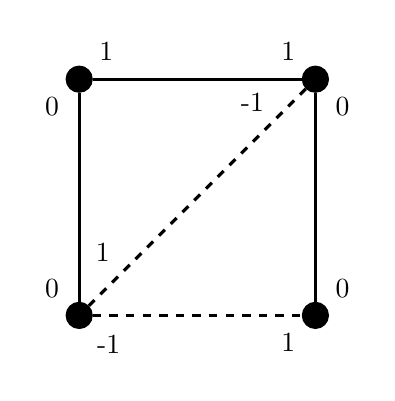
\begin{tikzpicture}
        \begin{scope}[every node/.style={circle,draw,fill=black}]
            \node (1) [label=above right:1, label=below left:0] at (0,0) {};
            \node (2) [label=above left:1, label=below right:0] at (3,0) {};
            \node (3) [label=above left:0, label=below right:-1] at (0,-3) {};
            \node (4) [label=above right:0, label=below left:1] at (3,-3) {};
        \end{scope}
        \node (ar) at (2.2,-0.3) {-1};
        \node (bl) at (0.3, -2.2) {1};
        \begin{scope}[every edge/.style={draw,very thick}]
            \path
                (1) edge (2)
                (2) edge [dashed] (3)
                (3) edge (1)
                (2) edge (4)
                (3) edge [dashed] (4);
        \end{scope}
    \end{tikzpicture}
    \hspace{0.1\textwidth}
    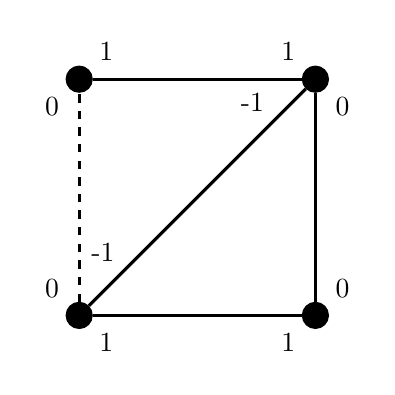
\begin{tikzpicture}
        \begin{scope}[every node/.style={circle,draw,fill=black}]
            \node (1) [label=above right:1, label=below left:0] at (0,0) {};
            \node (2) [label=above left:1, label=below right:0] at (3,0) {};
            \node (3) [label=above left:0, label=below right:1] at (0,-3) {};
            \node (4) [label=above right:0, label=below left:1] at (3,-3) {};
        \end{scope}
        \node (ar) at (2.2,-0.3) {-1};
        \node (bl) at (0.3, -2.2) {-1};
        \begin{scope}[every edge/.style={draw,very thick}]
            \path
                (1) edge (2)
                (2) edge [] (3)
                (3) edge [dashed] (1)
                (2) edge (4)
                (3) edge [] (4);
        \end{scope}
    \end{tikzpicture}
    \caption[Example of a signed edge colouring]{Example of a proper signed edge colouring on the left. We obtain the graph on the right by switching the bottom left vertex and the colouring remains correct and proper.}
\end{figure}

\section{Motivation}

\say{In the study of various important and difficult problems in graph theory (such as the cycle double cover conjecture and the 5-flow conjecture), one encounters an interesting but somewhat mysterious variety of graphs called snarks. In spite of their simple definition [\dots] and over a century long investigation, their properties and structure are largely unknown.} --- Chladný, Škoviera \cite{skoviera-citat}

By Vizing's theorem, cubic graphs are edge-colourable either with three ("class one" graphs) or four colours ("class two" graphs). The exact definition of a snark may vary from paper to paper but a snark is essentially a cubic graph with chromatic index four (its edges can't be coloured with three colours). Every cubic graph with a loop or a bridge is a "snark", triangles (cycles of length three) can be contracted into a single vertex and cycles of length four can also be simplified. Therefore many definitions forbid these properties by considering true snarks only graphs with girth (length of the shortest cycle) at least five. Even more strongly, only cyclically 4-edge-connected graphs are considered (there is no subset of three or fewer edges such that their removal will disconnect the graph into two subgraphs each containing a cycle). One of the alternative formulations of the four colour theorem is that each snark is non-planar. Snarks are important in a multitude of graph theory areas and thus it makes sense to investigate the reach of signed snarks too.

\section{Previous research}

In \textit{The chromatic number of a signed graph}\cite{chromatic-number} Máčajová et al. continue Zaslavsky's research by studying the properties of the chromatic number of signed graphs, ultimately proving a signed version of the famous Brooks'\cite{brooks} theorem.

\begin{theorem}[Signed Brooks' Theorem]\label{th:brooks}
    Let $\Gamma$ be a simple connected signed graph. If $\Gamma$ is not a balanced complete graph, a balanced odd circuit or an unbalanced even circuit, then $\chi(\Gamma) \leq \Delta(\Gamma)$.
\end{theorem}

\textit{Edge colouring signed graphs} defines a version of the signed edge colouring and proves a signed version of the equally fundamental Vizing's theorem.

\begin{theorem}[Signed Vizing's Theorem]\label{th:vizing}
    Let $\Gamma$ be a simple signed graph. The chromatic index of $\Gamma$ is $\Delta(\Gamma)$ or $\Delta(\Gamma) + 1$.
\end{theorem}
